%%%%%%%%%%%%%%%%%%%%%%%%%%%%%%%%%
%
% Lecture notes for Numerical Methods for Partial Differential Equations
%
% Chapter 3: Elliptic PDEs
%
%%%%%%%%%%%%%%%%%%%%%%%%%%%%%%%%%

% !TeX root = NumPDE_Lecture_notes.tex

\section{Elliptic partial differential equations}

\subsection{Finite-difference scheme for Poisson equation}

We will illustrate the finite-difference
method for elliptic PDEs with the Poisson equation
\begin{equation}
\Delta u = f(x,y)   \label{g1}
\end{equation}
for $(x,y)\in{\cal D}$ and
\begin{equation}
u(x,y) = g(x,y) \quad \hbox{for} \quad (x,y)\in S,   \label{g2}
\end{equation}
where
\[
\Delta\equiv\frac{\pr^{2}}{\pr x^{2}}+ \frac{\pr^{2}}{\pr y^{2}}, \quad
{\cal D}=\{\, (x,y)\, \vert \,  a<x<b, \ c<y<d \, \},
\]
and $S$ is the boundary of ${\cal D}$. In what follows, we assume that both
$f$ and $g$ are continuous
in ${\cal D}$ and that a unique solution of
the boundary-value problem (\ref{g1}), (\ref{g2}) exists.


 
The first step in the finite-difference method is to choose integers $N_{1}$ and $N_{2}$ and define
step sizes $h_{1}$ and $h_{2}$ by $h_{1}=(b-a)/N_{1}$ and $h_{2}=(d-c)/N_{2}$. Partitioning of
the interval $[a, b]$ into $N_{1}$ equal parts of width $h_{1}$ and
the interval $[c, d]$ into $N_{2}$ equal parts of width $h_{2}$ provides a grid on the
rectangle ${\cal D}$ by drawing vertical and horizontal lines through the points with coordinates
$(x_{k}, y_{j})$ where $x_{k}=a+kh_{1}$ for each $k=0,1,\dots,N_{1}$ and
$y_{j}=c+jh_{2}$ for each $j=0,1,\dots,N_{2}$.
 
Let $w_{kj}$ be an approximation to $u(x_{k}, y_{j})$.
For the interior mesh points $(x_{k}, y_{j})$ (with
$k=1,2,\dots,N_{1}-1$ and $j=1,2,\dots,N_{2}-1$), we approximate
the second partial derivatives with respect to $x$ and $y$
by the three-point central-difference formulas. As a result, we obtain the following
difference equations:
\[
\frac{w_{k+1,j}-2w_{k,j}+w_{k-1,j}}{h_{1}^{2}}+
\frac{w_{k,j+1}-2w_{k,j}+w_{k,j-1}}{h_{2}^{2}}=f_{kj}
\]
for each $k=1,2,\dots,N_{1}-1$ and $j=1,2,\dots,N_{2}-1$.
Here $f_{kj}=f(x_{k}, y_{j})$. Equivalently, we can rewrite
this as
\begin{equation}
2\left[1+\left(\frac{h_{1}}{h_{2}}\right)^{2}\right]w_{kj}-\left(w_{k+1,j}+w_{k-1,j}\right)
-\left(\frac{h_{1}}{h_{2}}\right)^{2}\left(w_{k,j+1}+w_{k,j-1}\right)
=-h_{1}^{2}f_{kj}, \label{g3}
\end{equation}
for each $k=1,2,\dots,N_{1}-1$ and $j=1,2,\dots,N_{2}-1$,
The boundary conditions at the
exterior mesh points yield
\begin{eqnarray}
&&w_{0,j}=g(x_{0}, y_{j}), \quad w_{N_{1},j}=g(x_{N_{1}}, y_{j})
\quad \hbox{for each} \quad j=1,\dots,N_{2}-1 \label{g4} \\
&&w_{k,0}=g(x_{k}, y_{0}), \quad w_{k,N_{2}}=g(x_{k}, y_{N_{2}})
\quad \hbox{for each} \quad k=1,2,\dots,N_{1}-1.\nonumber  
\end{eqnarray}
Note that we did not specify the approximations $w_{0,0}$,
$w_{N_{1},0}$, $w_{N_{1},N_{2}}$ and $w_{0,N_{2}}$ corresponding to
the vertices of the rectangle ${\cal D}$, because these points take
no part in Eq. (\ref{g3}).

 
Evidently, the local truncation
error of the finite difference method, given by (\ref{g3})--(\ref{g4}), is $O(h_{1}^{2}+h_{2}^{2})$).

 
The typical equation in (\ref{g3}) involves approximations to $u(x_{k}, y_{j})$ at the five
points
\[
(x_{k-1}, y_{j}), \quad (x_{k}, y_{j}), \quad (x_{k+1}, y_{j}), \quad
(x_{k}, y_{j-1}), \quad (x_{k}, y_{j+1}).
\]
If we use the information from the boundary conditions (\ref{g4})
whenever appropriate in the system (\ref{g3}), we have an
$(N_{1}-1)(N_{2}-1)$ by $(N_{1}-1)(N_{2}-1)$ linear system with
the unknowns $w_{ij}$ at the interior mesh points.

 
For simplicity, consider the square domain ($c=a$, $d=b$) with the same number of grid lines
in $x$ and $y$. Then $N_{1}=N_{2}\equiv N$ and $h_{1}=h_{2}\equiv h$. Equation (\ref{g3})
takes the form
\begin{equation}
4w_{k,j}-\left(w_{k+1,j}+w_{k-1,j}+w_{k,j+1}+w_{k,j-1}\right)
=-h^{2}f_{k,j}, \label{g5}
\end{equation}
for each $k,j=1,2,\dots,N-1$.

 
\begin{example}
Consider the boundary value problem
\begin{eqnarray}
&&\Delta u = f(x,y) \quad {\rm for} \quad 0< x< 1, \ \ 0< y< 1;  \nonumber \\
&&u(0,y)=0, \quad u(1,y)=1 \quad {\rm for} \quad 0< y< 1;  \nonumber \\
&&u(x,0)=x, \quad u(x,1)=x \quad {\rm for} \quad 0< x< 1.  \nonumber
\end{eqnarray}
Let $N=3$, so that $h=1/3$ and $x_{1}=y_{1}=1/3$, $x_{2}=y_{2}=2/3$.
Equations (\ref{g4}) become
\begin{eqnarray}
&&w_{0,1}=w_{0,2}=0, \quad w_{3,1}=w_{3,2}=1, \nonumber \\
&&w_{1,0}=w_{1,3}=x_{1}, \quad w_{2,0}=w_{2,3}=x_{2}. \label{g6}
\end{eqnarray}
Equations (\ref{g5}) take the form
\begin{eqnarray}
&&4w_{1,1}-\left(w_{2,1}+w_{0,1}+w_{1,2}+w_{1,0}\right)=-h^2f_{1,1}, \nonumber \\
&&4w_{2,1}-\left(w_{3,1}+w_{1,1}+w_{2,2}+w_{2,0}\right)=-h^2f_{2,1}, \nonumber \\
&&4w_{1,2}-\left(w_{2,2}+w_{0,2}+w_{1,3}+w_{1,1}\right)=-h^2f_{1,2}, \nonumber \\
&&4w_{2,2}-\left(w_{3,2}+w_{1,2}+w_{2,3}+w_{2,1}\right)=-h^2f_{2,2}, \nonumber
\end{eqnarray}
Substitution of (\ref{g6}) in these equations yields the system
\begin{equation}
\left(
\begin{array}{cccc}
4 &-1 &-1 &0 \\
-1 &4 &0 &-1 \\
-1 &0 &4 &-1 \\
0 &-1 &-1 &4
\end{array}\right)
\left(
\begin{array}{c}
w_{1,1} \\
w_{2,1} \\
w_{1,2} \\
w_{2,2}
\end{array}\right)=
\left(
\begin{array}{c}
x_{1}-h^2f_{1,1} \\
1+x_{2}-h^2f_{2,1} \\
x_{1}-h^2f_{1,2} \\
1+x_{2}-h^2f_{2,2}
\end{array}\right). \label{g7}
\end{equation}
Thus, our problem is reduced to solving system (\ref{g7})
of 4 linear equations for 4 unknowns.
\end{example}
 
In general, if we let
\begin{equation}
{\bf w}=\left[
\begin{array}{c}
w_{1,1} \\
w_{2,1} \\
\vdots \\
w_{N-1,1} \\
w_{1,2} \\
w_{2,2} \\
\vdots \\
w_{N-1,2} \\
w_{1,3} \\
\vdots \\
\vdots \\
w_{N-1,N-1}
\end{array}\right],
\quad {\bf f}=\left[
\begin{array}{c}
w_{0,1}+w_{1,0}-h^{2}f_{1,1} \\
w_{2,0}-h^{2}f_{2,1} \\
\vdots \\
w_{N-1,0}+w_{N,1}-h^{2}f_{N-1,1} \\
w_{0,2}-h^{2}f_{1,2} \\
-h^{2}f_{22}\\
\vdots \\
w_{N,2}-h^{2}f_{N-1,2} \\
w_{0,3}-h^{2}f_{1,3} \\
\vdots \\
\vdots \\
w_{N,N-1}+w_{N-1,N}-h^{2}f_{N-1,N-1}
\end{array}\right],
\label{g8}
\end{equation}
then the linear system (\ref{g5}) can be written in the matrix form
\begin{equation}
A{\bf w}={\bf f}, \label{g9}
\end{equation}
where
\begin{equation}
A=\left[
\begin{array}{cccccc}
A_{1} &B &0      &\dots  &\dots &0 \\
B &A_{1} &B &\ddots  &     &\vdots \\
0      &B &A_{1} &B &\ddots &\vdots \\
\vdots &\ddots &\ddots &\ddots &\ddots &0 \\
\vdots &       &\ddots &\ddots &\ddots &B \\
0      &\dots  &\dots  &0      &B &A_{1}
\end{array}\right], \label{g10}
\end{equation}
and where $A_{1}$ and $B$ are $(N-1)\times(N-1)$ matrices having the form
\begin{equation}
A_{1}=\left[
\begin{array}{cccccc}
4 &-1  &0      &\dots  &\dots &0 \\
-1 &4  &-1     &\ddots  &     &\vdots \\
0  &-1 &4      &-1      &\ddots &\vdots \\
\vdots &\ddots &\ddots &\ddots &\ddots &0 \\
\vdots &       &\ddots &\ddots &\ddots &-1 \\
0      &\dots  &\dots  &0      &-1 &4
\end{array}\right], \quad
B=-I=\left[
\begin{array}{cccc}
-1  &0      &\dots  &0 \\
0   &\ddots  &\ddots  &\vdots \\
\vdots  &\ddots  &\ddots  &0 \\
0     &\dots &0  &-1
\end{array}\right]. \label{g11}
\end{equation}
Thus, we have the linear algebraic system (\ref{g9}) with
the block-tridiagonal matrix $A$. Now we need
to answer two questions: (i) does system (\ref{g9}) have a unique solution and (ii) how to solve
(\ref{g9}) in practice?



\subsection{Existence of a unique solution of the finite-difference equations} 

The existence of a unique solution of the system $A{\bf w}={\bf f}$  is equivalent to non-existence of nontrivial
(i.e. nonzero) solutions of the homogeneous equation
\[
A{\bf w}=0.
\]
To show this non-existence, we will use the maximum principle. The equation can be written as
\begin{equation}
4w_{kj}-\left(w_{k+1,j}+w_{k-1,j}+w_{k,j+1}+w_{k,j-1}\right)
=0, \label{g12}
\end{equation}
for each $k,j=1,2,\dots,N-1$.  Equation (\ref{g12}) are supplemented with homogeneous
boundary conditions
\begin{equation}
w_{0j}=w_{N,j}=0 \quad \hbox{for} \quad j=0,1,\dots,N \quad \hbox{and} \quad
w_{k0}=w_{k,N}=0\label{g13}
\end{equation}
for $k=1,2,\dots,N-1$.
Let $(m,n)$ be a point at which the maximum of $w_{kj}$ is attained. There may be several points at
which the maximum is attained. If the maximum is attained at a boundary point then
$\max_{0\leq k,j\leq N}w_{kj}=0$.
Assume that the maximum is attained at an interior point $(m,n)$. Since, again,
there may be several such points, we choose a point $(m,n)$ such than
it corresponds to the maximum value of index $m$, i.e.
\[
w_{m,n}=\max_{0\leq k,j\leq N}w_{kj} \quad \hbox{and} \quad
w_{m,n}>w_{m+1,n}.
\]
Then the left-hand side of Eq. (\ref{g12}) at this maximum point will be strictly positive:
\begin{multline}
4w_{mn}-\left(w_{m+1,n}+w_{m-1,n}+w_{m,n+1}+w_{m,n-1}\right)\\
=w_{mn}-w_{m+1,n}+(w_{mn}-w_{m-1,n})+(w_{mn}-w_{m,n+1})+(w_{mn}-w_{m,n-1})\\
\geq w_{mn}-w_{m+1,n} > 0. \label{g14}
\end{multline}
Evidently, (\ref{g14}) is in contradiction with (\ref{g12}). Thus, our assumption that the maximum
is attained at an interior mesh point is wrong. Thus, we have
\begin{equation}
\max_{0\leq k,j\leq N}w_{kj}=0. \label{g15}
\end{equation}
Similarly, it can be shown that
\begin{equation}
\min_{0\leq k,j\leq N}w_{kj}=0. \label{g16}
\end{equation}
It follows from Eqs. (\ref{g15}) and (\ref{g16}) that $w_{kj}=0$ for
each $k,j=1,2,\dots,N-1$. Thus, the homogeneous system has only
zero solution, which proves that system $A{\bf w}={\bf f}$ has a unique
solution.


The maximum principle can also be used
to prove the convergence of the discrete approximations $w_{kj}$ to the solution. Namely, it is shown
in Appendix A that if $u\in C^{4}(D)$ (where $D=\{(x,y)\, \vert \ 0<x<1, \ 0<y<1 \, \}$)
is the exact solution of the boundary-value
problem
\begin{eqnarray}
&&u_{xx}+u_{yy} = f(x,y), \quad 0<x<1, \ \ 0<y<1;     \label{gg1} \\
&&u(0,y) = u(1,y) = 0, \quad
u(x,0) =u(x,1) = 0.   \label{gg2}
\end{eqnarray}
and $w_{kj}$ ($k,j=1,2, \dots,N-1$) satisfy
\begin{equation}
4w_{k,j}-\left(w_{k+1,j}+w_{k-1,j}+w_{k,j+1}+w_{k,j-1}\right)
=-h^{2}f_{k,j}, \label{gg5}
\end{equation}
for each $k,j=1,2,\dots,N-1$, then
\[
\left\vert w_{kj}-u(x_{k}, y_{j})\right\vert \leq Ah^{2},
\]
where $A$ is independent of $h$.



\subsection{Iterative techniques for solving the finite-difference equations}
For large systems ($N\gg 1$), an iterative
method (e.g., the Jacobi method, the Gauss-Seidel method or the SOR method) should
be used to solve system (\ref{gg5}). All these methods can be viewed as {\it relaxation methods}.
Consider the heat equation
\begin{equation}
\frac{\pr u}{\pr t}=\frac{\pr^2 u}{\pr x^2}+\frac{\pr^2 u}{\pr y^2} - f(x,y),   \label{g17}
\end{equation}
subject to boundary conditions (\ref{gg2}). An initial distribution $u_{0}(x,y)$ will {\it relax} to
an equilibrium solution as $t\to\infty$, and this equilibrium solution will be the solution of the
original elliptic problem (\ref{gg1}), (\ref{gg2}).


Suppose that to solve (\ref{g17}) we employ the explicit forward-difference scheme
\begin{equation}
\frac{w_{kj}^{n+1}-w_{kj}^{n}}{\tau} -\frac{1}{h^2}\left(
\delta_{x}^2+\delta_{y}^2\right)w_{kj}^{n}=-f_{kj}. \label{g18}
\end{equation}
We want to obtain an approximation to $u(x,y,T)$ where $T$ is as large as possible,
so we need to choose the step size in time $\tau$ at large as possible. We know that the
scheme (\ref{g18}) is stable only if $\tau/h^2\leq 1/4$, so we choose
\[
\tau=\frac{h^2}{4}.
\]
Substituting this in (\ref{g18}), we can rewrite it in the form
\begin{equation}
w_{kj}^{n+1}=\frac{1}{4}\left(w^{n}_{k+1,j}+w^{n}_{k-1,j}+w^{n}_{k,j+1}+w^{n}_{k,j-1}\right)
-\frac{h^2}{4}f_{kj}. \label{g19}
\end{equation}
This represent the Jacobi iterative technique for solving
linear system (\ref{gg5}).


Another classical method, the Gauss-Seidel method, is obtained from Eq. (\ref{g19})
by using $w_{kj}^{n+1}$ as soon as they become available. This leads to the formula
\begin{equation}
w_{kj}^{n+1}=\frac{1}{4}\left(w^{n}_{k+1,j}+w^{n+1}_{k-1,j}+w^{n}_{k,j+1}+w^{n+1}_{k,j-1}\right)
-\frac{h^2}{4}f_{kj}. \label{g20}
\end{equation}
Both the Jacobi and Gauss-Seidel methods are slowly converging and rarely used in practice.
A more appropriate method is the successive over-relaxation (SOR) method.

Another relaxation method for solving problem (\ref{gg1})--(\ref{gg2}) is to employ the alternating direction
implicit (ADI) method to solve the two-dimensional heat equation (\ref{g17}).
We know that this method is unconditionally stable, so that
there is no restriction of the step size in time. It can be shown however that the convergence of the
solution to the equilibrium solution is slower for large $\tau$, so we cannot let it be too large.
There exists an optimal value of $\tau$ and it can be shown that for large $N$ it is given by the formula
\[
\tau\approx\frac{1}{\pi}\frac{L^2}{N},
\]
where $L$ is the size of the (square) domain ${\cal D}$. Note that the time step corresponding
to the Jacobi method is much smaller (for large $N$) and is given by
\[
\tau=\frac{h^2}{4}=\frac{L^2}{4N^2}.
\]


\subsection{Double sweep method for solving the finite-difference equations}
To describe a direct (rather than iterative) methods for solving Eq. (\ref{gg5}), we rewrite
it in the form
\begin{eqnarray}
&&A_{1}{\bf v}_{1}+B{\bf v}_{2}={\bf f}_{1}, \nonumber \\
&&B{\bf v}_{1}+A_{1}{\bf v}_{2}+B{\bf v}_{3}={\bf f}_{2}, \nonumber \\
&& \dots \dots \dots \dots \dots \dots \dots \dots \dots \dots \dots \nonumber \\
&&B{\bf v}_{k-1}+A_{1}{\bf v}_{k}+B{\bf v}_{k+1}={\bf f}_{k}, \nonumber \\
&& \dots \dots \dots \dots \dots \dots \dots \dots \dots \dots \dots \nonumber \\
&&B{\bf v}_{N-2}+A_{1}{\bf v}_{N-1}={\bf f}_{{N-1}}, \label{g21}
\end{eqnarray}
where ${\bf v}_{k}$ is the vector with components $w_{1,k},
w_{2,k}, \dots, w_{N-1,k}$.
We can solve these equations with
the matrix form of the double-sweep method described below.


\textbf{Matrix double-sweep method.}
Consider the following system:
\begin{equation}
A_{i}\vv_{i-1}-C_{i}\vv_{i}+B_{i}\vv_{i+1}={\bf F}_{i} \quad \hbox{for}\quad i=1, \dots, N-1;
\quad \vv_{0}={\vV_{0}}, \ \ \vv_{N}={\vV_{N}} \label{yy22}
\end{equation}
where the coefficients $A_{i}$, $B_{i}$ and $C_{i}$ are given $(N-1)\times(N-1)$ real matrices,
${\bf F}_{i}, {\vV_{0}}, {\vV_{N}}\in\mathbb{R}^{N-1}$ are given vectors and $\vv_{i}\in\mathbb{R}^{N-1}$ are unknowns.

Let
\begin{equation}
\vv_{i-1}=\alpha_{i}\vv_{i}+\beta_{i}  \quad  \hbox{for} \quad
i=1, 2, \dots, N, \label{yy23}
\end{equation}
where $\alpha_{i}$ are $(N-1)\times(N-1)$ real matrices
and $\beta_{i}\in\mathbb{R}^{N-1}$.

Eliminating $\vv_{i-1}$, we find
\[
(A_{i}\alpha_{i}-C_{i})v_{i}+B_{i}v_{i+1}+A_{i}\beta_{i} - {\bf F}_{i}=0 \quad \hbox{for}\quad i=1, \dots, N-1.
\]
We also have
\[
\vv_{i}=\alpha_{i+1}\vv_{i+1}+\beta_{i+1}  \quad  \hbox{for} \quad
i=0, 1, \dots, N-1.
\]
Using this to eliminate $\vv_{i}$, we obtain
\[
[(A_{i}\alpha_{i}-C_{i})\alpha_{i+1}+B_{i}]\vv_{i+1}+[
(A_{i}\alpha_{i}-C_{i})\beta_{i+1}+A_{i}\beta_{i}-{\bf F}_{i}]=0 \quad \hbox{for}\quad i=1, \dots, N-1.
\]
This equation is satisfied if the two expressions in the square brackets are both zero:
\[
(A_{i}\alpha_{i}-C_{i})\alpha_{i+1}+B_{i}=O \quad \textrm{and} \quad
(A_{i}\alpha_{i}-C_{i})\beta_{i+1}+A_{i}\beta_{i}-{\bf F}_{i}=\mathbf{0}
\]
for $i=1, \dots, N-1$.

Therefore,
\begin{equation}
\alpha_{i+1}=-(A_{i}\alpha_{i}-C_{i})^{-1}B_{i}, \quad
\beta_{i+1}=(A_{i}\alpha_{i}-C_{i})^{-1}({\bf F}_{i}-A_{i}\beta_{i}) \quad
 \label{yy26}
\end{equation}
for $i=1, \dots, N-1$.

If $\alpha_{1}$ and  $\beta_{1}$ are known, then $\alpha_{i}$ and  $\beta_{i}$ for $i=2, 3, \dots, N$
can be computed using (\ref{yy26}). Formulae (\ref{yy26}) are well defined provided
$A_{i}\alpha_{i}-C_{i}$
is a nonsingular matrix for all $i$.

$\alpha_{1}$ and  $\beta_{1}$ can be determined as follows:
\[
\vv_{0}= \alpha_{1}\vv_{1}+\beta_{1} \quad \hbox{and} \quad \vv_{0}=\vV_{0} \quad \Rightarrow \quad
\alpha_{1}\vv_{1}+\beta_{1}=\vV_{0}.
\]
To satisfy this, we choose
\[
\alpha_{1}=O \quad \textrm{and} \quad \beta_{1}=\vV_{0}.
\]
Once we know all $\alpha_{i}$
and $\beta_{i}$, we compute $\vv_{N-1}, \vv_{N-2}, \dots, \vv_{1}$ using formula (\ref{yy23}).
This method works in practice but requires $N-1$ inversion of $(N-1)\times(N-1)$ matrices which
can be quite expensive computationally.

%\subsection{Cyclic reduction method}
%Consider now another direct method which is
%called the {\bf cyclic reduction} (CR) method. The idea of the method is as follows.
%Recalling that $B=-I$, we obtain [from (\ref{g21})]
%\begin{eqnarray}
%&&-{\bf v}_{k-2}+A_{1}{\bf v}_{k-1}-{\bf v}_{k}={\bf f}_{k-1}, \label{g22} \\
%&&-{\bf v}_{k-1}+A_{1}{\bf v}_{k}-{\bf v}_{k+1}={\bf f}_{k}, \label{g23} \\
%&&-{\bf v}_{k}+A_{1}{\bf v}_{k+1}-{\bf v}_{k+2}={\bf f}_{k+1}. \label{g24}
%\end{eqnarray}
%On multiplying Eq. (\ref{g23}) by $A_{1}$ and then adding the three equations, we obtain
%\begin{equation}
%-{\bf v}_{k-2}+A_{1}^{(1)}{\bf v}_{k}-{\bf v}_{k+2}={\bf f}^{(1)}_{k}, \label{g25}
%\end{equation}
%where
%\[
%A_{1}^{(1)}=A_{1}^{2}-2I, \quad {\bf f}^{(1)}_{k}={\bf f}_{k-1}+A_{1}{\bf f}_{k}+{\bf f}_{k+1}.
%\]
%This is an equation of the same form as Eq. (\ref{g23}). Thus, after one level of CR, we have
%reduced the number of equations by a factor of two. Since the resulting equation is of the same
%form as the original equation, we can repeat the procedure. Taking the number of points to
%be a power of $2$, say $N=2^m$, we, after $(m-1)$ steps, end up with a single equations for
%the central line of variables:
%\begin{equation}
%A_{1}^{(m-1)}{\bf v}_{N/2}={\bf f}^{(m-1)}_{N/2}+{\bf v}_{0}+{\bf v}_{N}, \label{g26}
%\end{equation}
%Here $A_{1}^{(m-1)}=\left[A_{1}^{(m-2)}\right]^2-2I$.
%Equation (\ref{g26}) represents a linear system with matrix $A_{1}^{(m-1)}$, which can be solved, e.g.,
%by the Gaussian elimination. At step $(m-2)$ we solve two linear systems
%\[
%A_{1}^{(m-2)}{\bf v}_{N/4}={\bf f}^{(m-2)}_{N/4}+{\bf v}_{0}+{\bf v}_{N/2} \quad {\rm and}
%\quad
%A_{1}^{(m-2)}{\bf v}_{3N/4}={\bf f}^{(m-2)}_{3N/4}+{\bf v}_{N/2}+{\bf v}_{N}.
%\]
%At step $(m-3)$ we solve four linear systems similar to these, etc. In total, we have to solve
%$N-1$ linear system.


 
\subsection{Neumann boundary conditions} 
Consider the Laplace equation
\begin{equation}
u_{xx}+u_{yy} =0    \label{gg101}
\end{equation}
in the unit square ($0<x<1, \ 0<y<1$) with boundary conditions for normal derivative
(Neumann problem):
\begin{equation}
u_{x}(0,y) =g_{0}(y), \quad u_{x}(1,y) =g_{1}(y), \quad u_{y}(x,0)=h_{0}(x), \quad
u_{y}(x,1) = h_{1}(x).    \label{gg102}
\end{equation}
At interior grid points $(x_{k},y_{j})$, $k,j=1,2,\dots,N-1$, we use the standard difference equations
\begin{equation}
4w_{k,j}-\left(w_{k+1,j}+w_{k-1,j}+w_{k,j+1}+w_{k,j-1}\right)
=0, \label{gg103}
\end{equation}
To approximate boundary conditions (\ref{gg102}),
we introduce false boundaries at $x=x_{-1}=-h$, $x=x_{N+1}=x_{N}+h$, $y=y_{-1}=-h$ and $y=y_{N+1}=y_{N}+h$
and the corresponding false grid points
$(x_{-1},y_{j})$, $(x_{N+1},y_{j})$ for $j=0,1,\dots,N$
and $(x_{k},y_{-1})$, $(x_{k},y_{N+1})$ for $k=0,1,\dots,N$.
Then we use the central difference formula for the 1st derivatives
with respect to $x$ and $y$ to approximate boundary condition (\ref{gg102}):
\begin{align*}
\frac{w_{1,j}-w_{-1,j}}{2h}&=g_{0}(y_j),  & \frac{w_{N+1,j}-w_{N-1,j}}{2h}&=g_{1}(y_j), \\
\frac{w_{k,1}-w_{k,-1}}{2h}&=h_{0}(x_k),  & \frac{w_{k,N+1}-w_{k,N-1}}{2h}&=h_{1}(x_k)
\end{align*}
or
\begin{align}
w_{-1,j}&=w_{1,j}-2h g_{0}(y_j), & w_{N+1,j}&=w_{N-1,j}+2h g_{1}(y_j), \notag\\
w_{k,-1}&=w_{k,1}-2h h_{0}(x_k), & w_{k,N+1}&=w_{k,N-1}+2h h_{1}(x_k). \label{p2b}
\end{align}
Assuming that Eq. (\ref{gg101}) is satisfies at the boundary, we extend Eq.  (\ref{gg103})
to the boundary grid points and use Eqs. (\ref{p2b})
to eliminate $w_{-1,j}$, $w_{N+1,j}$, $w_{k,-1}$ and $w_{N+1,j}$ wherever it is necessary. This yields
\begin{eqnarray}
&&4w_{0,j}-\left(2w_{1,j}+w_{0,j+1}+w_{0,j-1}\right)
=-2h g_{0}(y_j), \label{gg104} \\
&&4w_{N,j}-\left(2w_{N-1,j}+w_{N,j+1}+w_{N,j-1}\right)
=2h g_{1}(y_j), \label{gg105} \\
&&4w_{k,0}-\left(w_{k+1,0}+w_{k-1,0}+2w_{k,1}\right)
=-2h h_{0}(x_k), \label{gg106} \\
&&4w_{k,N}-\left(w_{k+1,N}+w_{k-1,N}+2w_{k,N-1}\right)
=2h h_{1}(x_k). \label{gg107}
\end{eqnarray}
Equations (\ref{gg103}) and (\ref{gg104})--(\ref{gg107}) represent the system of $(N+1)^2$
linear equations for $(N+1)^2$ unknowns $w_{kj}$ ($k,j=0,1,\dots,N$).
In vector form, we have
\[
A{\bf w}={\bf f}.
\]
However, it can be shown that matrix $A$ here is singular. This is a consequence of the fact
that the boundary value problem (\ref{gg101}), (\ref{gg102}) is solvable only under certain
condition (a solvability condition). Indeed, integrating Eq. (\ref{gg101}) over the unit square
and taking account of boundary conditions (\ref{gg102}), we obtain
\begin{equation}
\int\limits_{0}^{1}\int\limits_{0}^{1}
\left(u_{xx}+u_{yy}\right)dxdy=0 \quad \Rightarrow \quad
\int\limits_{0}^{1}(g_{1}(y)-g_{0}(y))dy+
\int\limits_{0}^{1}(h_{1}(x)-h_{0}(x))dx=0. \label{gg108}
\end{equation}
Thus, problem (\ref{gg101}), (\ref{gg102}) is solvable not for arbitrary functions
$g_{0,1}(y)$, $h_{0,1}(x)$ but only for functions that satisfy the solvability
condition (\ref{gg108}). Fortunately, many elliptic boundary value problems which
arise in practice do satisfy the solvability condition\footnote{Even in this case, the solution
is not unique: there are infinitely many solutions that differ one from another by a constant. Evidently,
if $u(x,y)$ is a solution of (\ref{gg101}), (\ref{gg102}), then $u(x,y)+c$ with any constant $c$ is also
a solution.}. So, if we know that a solution exists and want to find a numerical approximation to it,
we need to solve a system of linear algebraic equation with singular matrix. In this case, the direct methods
do not work. We may try to use iterative techniques described above. Sometimes this may work. But it is better
to use some different numerical technique (such as Galerkin method or finite-element method).




\subsection{Equations with variable coefficients}

Consider now the following elliptic equation
\begin{equation}
A(x,y)\frac{\pr^2 u}{\pr x^2}+B(x,y)\frac{\pr^2 u}{\pr y^2}+
C(x,y)\frac{\pr u}{\pr x}+D(x,y)\frac{\pr u}{\pr y}+F(x,y) \, u = G(x,y)
\label{h1}
\end{equation}
for $(x,y)\in{\cal D}$ where ${\cal D}=\{\, (x,y)\, \vert \,  a<x<b, \ c<y<d \, \}$ and
$A$, $B$, $C$, $D$, $F$ and $G$ are given functions of $x$ and $y$ in ${\cal D}$.
Equation (\ref{h1}) is supplemented with
the boundary conditions (at the boundary $S$ of the region ${\cal D}$):
\begin{equation}
u(x,y) = g(x,y) \quad \hbox{for} \quad (x,y)\in S.   \label{h2}
\end{equation}
To find a finite-difference approximation to the boundary value problem
(\ref{h1}), (\ref{h2}) at interior grid points $(x_{k},y_{j})$ ($x_{k}=a+h_{1}k$ for
$k=1,\dots,N_{1}$, $y_{j}=a+h_{2}j$ for
$j=1,\dots,N_{2}$, $h_{1}=(b-c)/N_{1}$, $h_{2}=(b-c)/N_{2}$), we use
the three-point central-difference formulas
to approximate the first and second partial derivatives with respect to $x$ and $y$
As a result, we obtain the following
difference equations:
\begin{equation}
\left(\frac{A_{kj}}{h_{1}^2}\delta_{x}^2+
\frac{B_{kj}}{h_{2}^2}\delta_{y}^2+ \frac{C_{kj}}{2h_{1}}\delta_{x}+
\frac{D_{kj}}{2h_{2}}\delta_{y}+F_{kj}\right)w_{kj}=G_{kj} \label{h3}
\end{equation}
where
\begin{align*}
\delta_{x}^2&=w_{k+1,j}-2w_{k,j}+w_{k-1,j}, &
\delta_{y}^2&=w_{k,j+1}-2w_{k,j}+w_{k,j-1}, \\
\delta_{x}&=w_{k+1,j}-w_{k-1,j}, &
\delta_{y}&=w_{k,j+1}-w_{k,j-1},
\end{align*}
and where $A_{kj}=A(x_{k},y_{j})$, $B_{kj}=B(x_{k},y_{j})$, etc.
Since the truncation error of each formula employed to obtain Eq. (\ref{h3})
is either $O(h_{1}^{2})$ or $O(h_{2}^{2})$, the truncation error of
this finite-difference method is $O(h_{1}^{2}+h_{2}^{2})$).

\vskip 0.3cm
 
If we use the information from the boundary conditions (\ref{h2})
whenever appropriate in the system (\ref{h3}), we obtain an
$(N_{1}-1)(N_{2}-1)$ by $(N_{1}-1)(N_{2}-1)$ linear system with
the unknowns $w_{ij}$ at the interior mesh points:
\[
A{\bf w}={\bf b}
\]
The matrix $A$ of this linear system is, in general, not symmetric even for
the square domain ($c=a$, $d=b$) with the same number of grid lines in $x$ and
$y$ because the coefficients of Eq. (\ref{h1}) depend on $x$ and $y$.

\vskip 0.3cm
 
If the linear elliptic equation (\ref{h1}) is self-adjoint or can be made
self-adjoint, i.e. can be written in the form
\[
\frac{\pr }{\pr x}\left(A\frac{\pr u}{\pr x}\right)+
\frac{\pr }{\pr y}\left(B\frac{\pr u}{\pr y}\right)
+F \, u = G,
\]
for some $A(x,y)$ and $B(x,y)$, and we have the square domain ($c=a$, $d=b$) with the same number of grid lines in $x$ and
$y$, then the symmetry of $A$ can be assured if we employ approximations of the form
\begin{eqnarray}
&&\frac{\pr }{\pr x}\left(A\frac{\pr u}{\pr x}\right)\biggm\vert_{(x_{k},y_{j})}=
\frac{A_{k+\frac{1}{2},j}}{h^2}\left(u_{k+1,j}-u_{k,j}\right)-
\frac{A_{k-\frac{1}{2},j}}{h^2}\left(u_{k,j}-u_{k-1,j}\right)+O(h^2), \nonumber \\
&&\frac{\pr }{\pr y}\left(B\frac{\pr u}{\pr y}\right)\biggm\vert_{(x_{k},y_{j})}=
\frac{B_{k,j+\frac{1}{2}}}{h^2}\left(u_{k,j+1}-u_{k,j}\right)-
\frac{B_{k,j-\frac{1}{2}}}{h^2}\left(u_{k,j}-u_{k,j-1}\right)+O(h^2), \nonumber
\end{eqnarray}
where $A_{k\pm\frac{1}{2},j}=(A_{k\pm 1,j}+A_{kj})/2$ and
$B_{k,j\pm\frac{1}{2}}=(B_{k,j\pm 1}+B_{kj})/2$.


%%%%%%%%%%%%%%%%%%%%%%%%%%%%%%%%%%%%%%%%%%%%%%%%%%%%%%%%%%%%%%%%%%%%%%%%%%%%%%%%%%%%%%%%%%%%%%%%%%%%%%%%%%%%%

%\subsection{Eigenvalues of differential operators}


%Consider
%the following eigenvalue problem for the Laplace operator:
%\begin{eqnarray}
%&&u_{xx}+u_{yy} = \lambda \, u  \quad {\rm for} \ \ 0< x < L_{1}, \ \ 0< y < L_{2}, \label{eig1} \\
%&&u(0,y) =u(L_{1},y)=0,\quad u(x,0)=u(x,L_{2})=0.   \label{eig2}
%\end{eqnarray}
%The problem is to find $\lambda$ (eigenvalue) such that there exists a nonzero solution (eigenfunction) of (\ref{eig1}) and (\ref{eig2}).

%\vskip 0.3cm
% 
%Introducing the standard grid ($(x_{k}, y_{j})=(k h_{1}, j h_{2})$ for $k=0,1,\dots,N_{1}$ and
%$j=0,1,\dots,N_{2}$ where $h_{1}=L_{1}/N_{1}$ and $h_{2}=L_{2}/N_{2}$) and employing the standard
%finite-difference formulae, we obtain the following
%difference equations:
%\[
%\frac{w_{k+1,j}-2w_{k,j}+w_{k-1,j}}{h_{1}^{2}}+
%\frac{w_{k,j+1}-2w_{k,j}+w_{k,j-1}}{h_{2}^{2}}= \lambda \, w_{kj}
%\]
%for each $k=1,2,\dots,N_{1}-1$ and $j=1,2,\dots,N_{2}-1$.
%These can be written in vector form as
%\begin{equation}
%A{\bf w}=\lambda \, {\bf w}, \label{eig3}
%\end{equation}
%where
%\begin{equation}
%A=\left[
%\begin{array}{cccccc}
%C &B &0      &\dots  &\dots &0 \\
%B &C &B &\ddots  &     &\vdots \\
%0      &B &C &B &\ddots &\vdots \\
%\vdots &\ddots &\ddots &\ddots &\ddots &0 \\
%\vdots &       &\ddots &\ddots &\ddots &B \\
%0      &\dots  &\dots  &0      &B &C
%\end{array}\right], \quad
%{\bf w}=\left[
%\begin{array}{l}
%w_{11} \\
%w_{21} \\
%\vdots \\
%w_{N_{1}-1,1} \\
%w_{12} \\
%\vdots \\
%w_{N_{1}-1,N_{2}-1}
%\end{array}\right],  \label{eig4}
%\end{equation}
%and where $C$ and $B$ are $(N_{1}-1)\times(N_{1}-1)$ matrices having the form
%\begin{equation}
%C=\left[
%\begin{array}{cccccc}
%-\frac{2}{h_{1}^2}-\frac{2}{h_{2}^2} &\frac{1}{h_{1}^2}  &0      &\dots  &\dots &0 \\
%\frac{1}{h_{1}^2} &-\frac{2}{h_{1}^2}-\frac{2}{h_{2}^2} &\frac{1}{h_{1}^2}     &\ddots  &     &\vdots \\
%0  &\frac{1}{h_{1}^2} &-\frac{2}{h_{1}^2}-\frac{2}{h_{2}^2}      &\frac{1}{h_{1}^2}      &\ddots &\vdots \\
%\vdots &\ddots &\ddots &\ddots &\ddots &0 \\
%\vdots &       &\ddots &\ddots &\ddots &\frac{1}{h_{1}^2} \\
%0      &\dots  &\dots  &0      &\frac{1}{h_{1}^2} &-\frac{2}{h_{1}^2}-\frac{2}{h_{2}^2}
%\end{array}\right], \quad
%B=\frac{1}{h_{2}^2} I=\left[
%\begin{array}{cccc}
%\frac{1}{h_{2}^2}   &0      &\dots  &0 \\
%0   &\ddots  &\ddots  &\vdots \\
%\vdots  &\ddots  &\ddots  &0 \\
%0     &\dots &0  &\frac{1}{h_{2}^2}
%\end{array}\right]. \label{g11}
%\end{equation}
%Thus, we reduced the original eigenvalue problem, given by (\ref{eig1}) and (\ref{eig2}), to
%the eigenvalue problem for matrix $A$. The latter can be solved by standard methods. In MATLAB,
%eigenvalues of matrix $A$ can be found using built-in MATLAB function {\bf eig}.

%\vskip 0.3cm
% 
%Generalisation of the above procedure to general second-order differential operators with variable coefficients
%is straightforward.



%%%%%%%%%%%%%%%%%%%%%%%%%%%%%%%%%%%%%%%%%%%%%%%%%%%%%%%%%%%%%%%%%%%%%%%%%%%%%%%%%%%%%%%%%%%%%%%%%%%%%%%%%%%%%

\subsection{Arbitrary (not rectangular) domains}

How to deal with the problem when region
${\cal D}$ is not a rectangle? In this case, we first cover the
whole region by a rectangular grid, say, with the step length
$h_{1}$ in the $x$ direction and the step length $h_{2}$ in the
$y$ direction. Then all interior grid points can be divided in two
groups: regular and irregular grid points. A grid point is called
regular if all its neighbouring grid points are also inside region
${\cal D}$. At a regular point, we can use the difference equation
(\ref{h3}). Irregular points require a special treatment.

\begin{figure}[h]
\centering
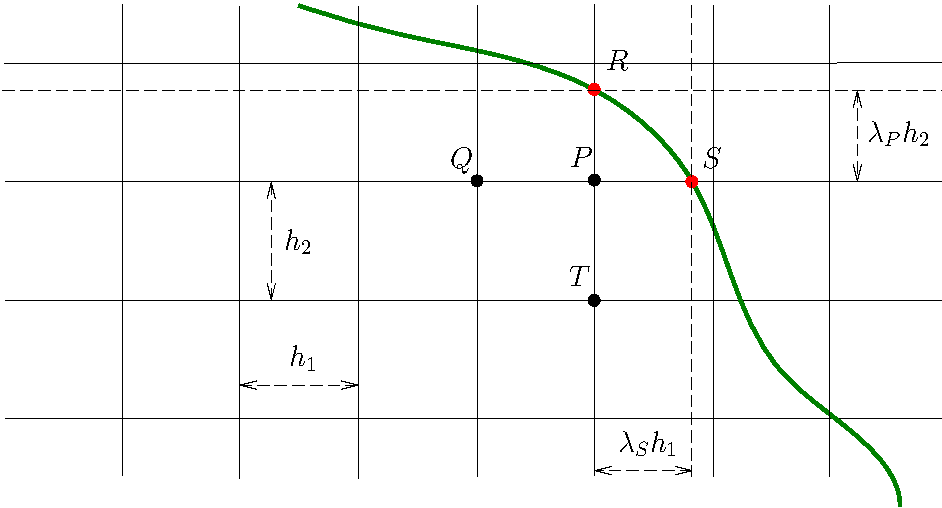
\includegraphics[width=11cm,height=8cm]{curved_bound_new.pdf}
\caption{}
\end{figure}

\vskip 0.3cm   Suppose that $P=(x,y)$ is an irregular grid
point, such that $S=(x+\lambda_{S}h_{1},y)$ and
$R=(x,y+\lambda_{R}h_{2})$ where $0<\lambda_{S,R}<1$ lie on the
boundary of ${\cal D}$ and the other two neighbouring grid points,
$Q=(x-h_{1},y)$ and $T=(x,y-h_{2})$, are inside ${\cal D}$ (see
Fig. 1). Then the derivatives of $u$ at point $P$ can be
approximated in the following manner. First, we expand
$u_{S}=u\vert_{S}$ and $u_{Q}=u\vert_{Q}$ in Taylor series at
point $P$:
\begin{eqnarray}
&&u_{S}=u_{P}+\lambda_{S}h_{1}\frac{\pr u}{\pr x}\biggm\vert_{P}+
\frac{(\lambda_{S}h_{1})^2}{2}\frac{\pr^2 u}{\pr x^2}\biggm\vert_{P}+O(h_{1}^3), \nonumber \\
&&u_{Q}=u_{P}-h_{1}\frac{\pr u}{\pr x}\biggm\vert_{P}+
\frac{h_{1}^2}{2}\frac{\pr^2 u}{\pr
x^2}\biggm\vert_{P}+O(h_{1}^3),  \nonumber
\end{eqnarray}
Multiplying the second equation by $\lambda_{S}^2$ and subtracting
the result from the first equation yields
\[
\frac{\pr u}{\pr
x}\biggm\vert_{P}=\frac{1}{h_{1}\lambda_{S}(1+\lambda_{S})} \left[
u_{S}-\lambda_{S}^2
u_{Q}-(1-\lambda_{S}^2)u_{P}\right]+O(h_{1}^2).
\]
Similarly, if we multiply the second equation by $\lambda_{S}$ and
add the result to the first equation yields, we can obtain the
formula for the second derivative with respect to $x$:
\[
\frac{\pr^2 u}{\pr
x^2}\biggm\vert_{P}=\frac{2}{h_{1}^2\lambda_{S}(1+\lambda_{S})}
\left[ u_{S}+\lambda_{S}
u_{Q}-(1+\lambda_{S})u_{P}\right]+O(h_{1}).
\]
Note that the truncation error of the formula for the second
derivative is $O(h_{1})$. To obtain a higher order accuracy, we
need to use one more grid point, e.g. point $(x-2h_1,y)$.

\vskip 0.3cm   Similarly, one can obtain the following
formulae for the derivatives with respect to $y$:
\begin{eqnarray}
&&\frac{\pr u}{\pr
y}\biggm\vert_{P}=\frac{1}{h_{2}\lambda_{R}(1+\lambda_{R})}
\left[ u_{R}-\lambda_{R}^2 u_{T}-(1-\lambda_{R}^2)u_{P}\right]+O(h_{2}^2), \nonumber \\
&&\frac{\pr^2 u}{\pr
y^2}\biggm\vert_{P}=\frac{2}{h_{2}^2\lambda_{R}(1+\lambda_{R})}
\left[ u_{R}+\lambda_{R}
u_{T}-(1+\lambda_{R})u_{P}\right]+O(h_{2}). \nonumber
\end{eqnarray}

